\documentclass[border=2pt]{standalone}



\usepackage{tikz}
\usetikzlibrary{matrix,positioning,arrows.meta,arrows,calc}
\tikzset{
mymat/.style={
  matrix of nodes,
  text height=2.5ex,
  text depth=0.75ex,
  text width=3.25ex,
  inner xsep=0ex,
  align=center,
  column sep=-\pgflinewidth,
  nodes={minimum width=4ex}
  }
}



\begin{document}



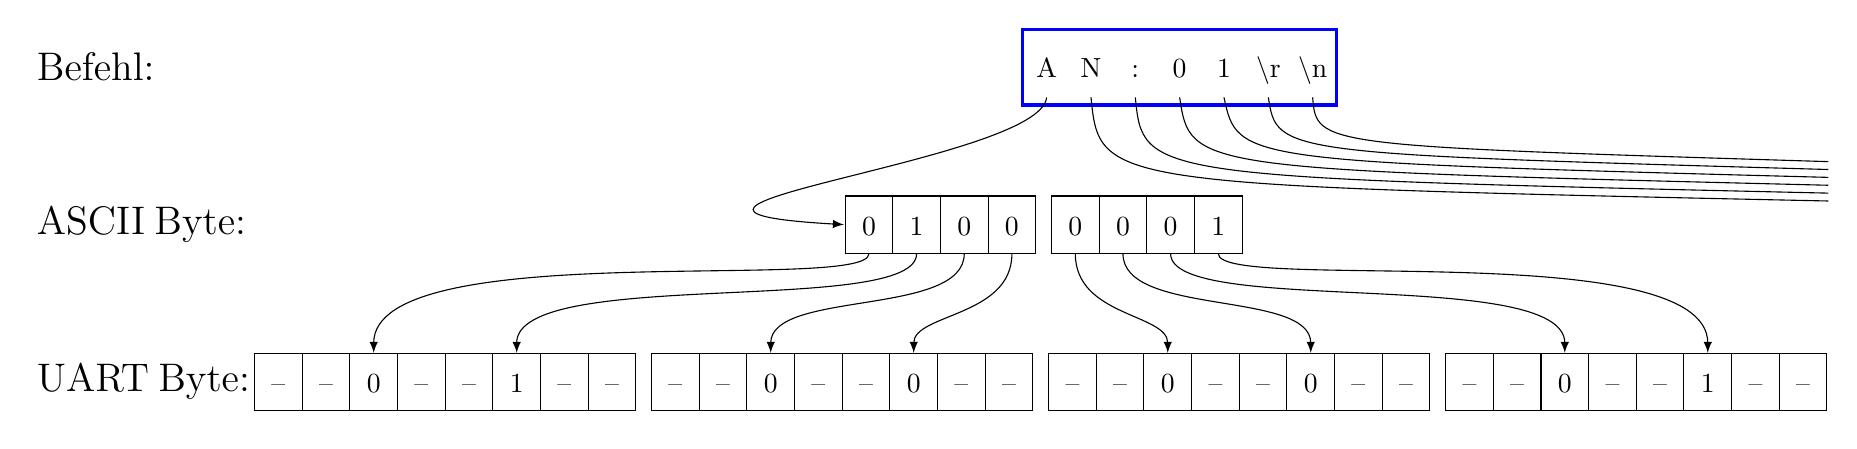
\begin{tikzpicture}[draw, minimum width=1cm, minimum height=0.5cm]
  \node[text width=3.5cm] at (-1, 3) {\Large Befehl:};
  \node[text width=3.5cm] at (-1, 1) {\Large ASCII Byte:};
  \node[text width=3.5cm] at (-1,-1) {\Large UART Byte:};

  \matrix[mymat,anchor=west,draw=blue,very thick] at (9.75,3) 
  (pc) {
    |(pos1)| A &
    |(pos2)| N &
    |(pos3)| : &
    |(pos4)| 0 &
    |(pos5)| 1 &
    |(pos6)| \textbackslash r &
    |(pos7)| \textbackslash n\\
  };

  \matrix[mymat,anchor=west,style={nodes=draw}] at (7.5,1) 
  (ASCII-a) {
          |(bit7)| 0 &
          |(bit6)| 1 &
          |(bit5)| 0 &
          |(bit4)| 0 &
    [2mm] |(bit3)| 0 &
          |(bit2)| 0 &
          |(bit1)| 0 &
          |(bit0)| 1 \\
  };

  \draw[-latex] (pos1.south) .. controls (10,1.8) and (4,1.2) .. (ASCII-a.west);
  \draw (pos2.south) .. controls (10.75,1.5) .. (20,1.3);
  \draw (pos3.south) .. controls (11.3,1.6) .. (20,1.4);
  \draw (pos4.south) .. controls (11.9,1.7) .. (20,1.5);
  \draw (pos5.south) .. controls (12.5,1.8) .. (20,1.6);
  \draw (pos6.south) .. controls (13,1.9) .. (20,1.7);
  \draw (pos7.south) .. controls (13.5,2.0) .. (20,1.8);
  
  
  
  \matrix[mymat,anchor=west,style={nodes=draw}] at (0,-1)
  (UART-coffee) {
          -- & -- & |(bit7uart)| 0 & -- & -- & |(bit6uart)| 1 & -- & -- &
    [2mm] -- & -- & |(bit5uart)| 0 & -- & -- & |(bit4uart)| 0 & -- & -- &
    [2mm] -- & -- & |(bit3uart)| 0 & -- & -- & |(bit2uart)| 0 & -- & -- &
    [2mm] -- & -- & |(bit1uart)| 0 & -- & -- & |(bit0uart)| 1 & -- & -- \\
  };

  \draw[-latex] (bit7.south) .. controls ($(bit7.south)+(0,-0.5)$) and ($(bit7uart.north)+(0,1.5)$) .. (bit7uart.north);
  \draw[-latex] (bit6.south) .. controls ($(bit6.south)+(0,-0.8)$) and ($(bit6uart.north)+(0,1.1)$) .. (bit6uart.north);
  \draw[-latex] (bit5.south) .. controls ($(bit5.south)+(0,-0.8)$) and ($(bit5uart.north)+(0,0.8)$) .. (bit5uart.north);
  \draw[-latex] (bit4.south) .. controls ($(bit4.south)+(0,-0.8)$) and ($(bit4uart.north)+(0,0.5)$) .. (bit4uart.north);
  \draw[-latex] (bit3.south) .. controls ($(bit3.south)+(0,-0.8)$) and ($(bit3uart.north)+(0,0.5)$) .. (bit3uart.north);
  \draw[-latex] (bit2.south) .. controls ($(bit2.south)+(0,-0.8)$) and ($(bit2uart.north)+(0,0.8)$) .. (bit2uart.north);
  \draw[-latex] (bit1.south) .. controls ($(bit1.south)+(0,-0.8)$) and ($(bit1uart.north)+(0,1.1)$) .. (bit1uart.north);
  \draw[-latex] (bit0.south) .. controls ($(bit0.south)+(0,-0.5)$) and ($(bit0uart.north)+(0,1.5)$) .. (bit0uart.north);

\end{tikzpicture}



\end{document}
